\section{Background}
\subsection{Private cars as a mode of transport in urban settings}
\justify

%--talking points in this subsection
%Donald Shoup searching for parking
%city congestion
%private car mobility
%amount of cars in urban settings
%the space parked cars take

% parking policy:
%Goals of parking policy are numerous, for example optimal accessibility and traffic flow and maximising turn-over for shops (\cite{Marsden2006}).
The number of private cars is globally on the rise. According to one estimation, the world reached one billion cars in 2020 (\cite{Sperling2009}). International Organization of Motor Vehicle Manufacturers (OICA) estimates, that we were already at 950 million private cars in 2015 (\cite{OICA2020}). As the production of private cars is expected to continue, eyes must turn to managing the vast quantity of personal transportation in cities and in their surroundings. This is a question of mitigation of climate change, but also ensuring the economic performance of cities, and maximising the quality of life for urban citizens (\cite{Bertolini2003}).

Since the last century, urban landscapes have experienced change toward car based mobility, where streets have incrementally widened and parking standards continually increased. Much of the time this space has been taken from all other users of public space to accommodate cars (\cite{Cervero2017}). As cars have become a most common sight in cities, the mitigation of their adverse effects have become an important focus in policy. A major challenge cities face today is the relation of mobility of people and the urban land use. It has been shown that parking policy is an effective tool in the management of this challenge (\cite{Diallo2015}; \cite{Marsden2006}).

One goal of parking policy is an urban environment less dependant on private cars. However, a central issue in attempting to shape urban development in a direction that's less dependent on cars is that the alternatives fail to reach the quality of accessibility provided by private cars (\cite{Bertolini2003}).

\newpage
\subsection{Accessibility}
\justify

Considering transportation of persons in cities, It may be thought that it is of highest priority to reach places as fast as possible. This is spatial mobility, movement which can be observed. However, people are ultimately not interested in measuring time units, but in social and economic interactions. It can then be said that the actual matter to focus in transporting persons in cities is not mobility, but accessibility. Accessibility can be defined as potential movement, observed through modeling. In accessibility, it is possible to attain a more realistic view into what is possible with available resources, such as time, and combine this matter with important issues regarding the sustainable development of cities. (\cite{Hodge1997}; \cite{Tenkanen2017}; \cite{Cervero2017})

First discussed by \citeauthor{Hansen1959} (\citeyear{Hansen1959}), accessibility as a concept has been widely studied in the decades that followed. In these first efforts Hansen succeeded in showing that locations in Washington D.C., United States, that had good accessibility were more likely to end up developed. These areas would also be developed at a higher density.

Torsten Hägerstrand's classic time geography approach developed further the idea that accessibility is a intricate complex of interdisciplinary tendencies. Individuals can be viewed as a bearers of action spaces of varying sizes and durations, which are determined by their social role, income, and how advanced technology they can access. Individuals are bound to their time budgets which are indivisible from certain constraints: the capacity, coupling, and institutional constraints (\cite{Wegener1999}; \cite{Hagerstrand1970}).

%Hodge asks how to navigate the intricate implications of accessibility, and reject the simplicity of distance or time as measure of accessibility (\cite{Hodge1997})
Continuing on Hägerstrand's action-space line of thinking, Zahavi (\citeyear{Zahavi1974}) proposed that individuals are not attempting to minimise travel time or cost required for a number of activities, but to maximise what is available to them considering their travel times and monetary budgets. Zahavi's theory can explain why the expansion of private car use has been as extensive as it has been. According to \citeauthor{Wegener1999} (\citeyear{Wegener1999}), the theory sheds light why the motorisation in the twentieth century caused even longer and more car trips when travel speed gains were attained and why shopping centers in outskirts of cities can attract customers from ever more larger areas of influence.

More recently, \citeauthor{Geurs2004} (\citeyear{Geurs2004}) and \citeauthor{Bertolini2003} (\citeyear{Bertolini2003}) have provided their definitions for accessibility. \citeauthor{Geurs2004} argues that accessibility should be associated with land use and transport systems in society and this would provide individuals with opportunities to take part in activities in different locations. According to \cite{Bertolini2003}, accessibility refers to the quantity and the diversity of spatial opportunities which can be reached within a certain amount of time.

\newpage
\subsection{Previous parking studies}
\justify
%Hyödynnä taustoittamisessa:
%\cite{Belloche2015}, On-street Parking Search Time Modelling and Validation with Survey-based Data
%\cite{Aryandoust2019}, City-scale car traffic and parking density maps from Uber Movement travel time data
%\cite{Axhausen1993}, Effectiveness of parking guidance and information systems: recent evidence from Nottingham and Frankfurt am Main
%\cite{Parmar2020}, Study on demand and characteristics of parking system in urban areas: A review

%\cite{VanDerGoot1982}: "A model to describe the choice of parking places". walking time greatly influenced the visitor's choice
Van der Goot (\cite{VanDerGoot1982}) walking time greatly influenced the visitor's choice
Van der Goot (\cite{VanDerGoot1982}) parking study in Haarlem
Van der Goot (\cite{VanDerGoot1982}) found out that a purpose of "shopping", longer walking times to destination led to longer parking times, and shorter walking times to shorter parking times.

An agent-based model designed to capture trip chaining behaviour and "often-overlooked" phenomenon of drivers searching for parking for an available spot (\cite{Guo2013}).
Parking search process: driver upon arriving to campus would first go to his/her most desirable lot on campus, only to find it full and would thus have to drive to his second-choice parking lot and so on until he/she finds an available spot  (\cite{Guo2013}).

Thompson and Richardson showed that long term experience does not necessarily lead to better choices in parking search (\cite{Thompson1998}).
adverse effects on traffic congestion (thompson 1998:ssa: parker 73, gillen 77, feeney 89)
Parking choice is a search process, where drivers make a number of linked decisions based on updated knowledge gained from experience (lukee thompsonissa 1998: layzell85, polak+axhausen89)
The parking search process figure (\cite{Thompson1998}).
Motorists must base their choice on imperfect information, synthesise the initial perception with the additional information gained from previous as well as the current searching experiences (\cite{Thompson1998}).

amount and location of parking affect 1) level of service and congestion on access roads and internal city streets, 2) efficiency, effectiveness and financial performance of public transport 3) amenity, safety and environmental integrity of the city and its surroundings, and 4) form and functioning of the metropolitan region as a whole (\cite{Young1991})

Parking search problems arise from mismatch between parking intentions of the travellers and supply (\cite{Axhausen1993}).
In some cases problems are because overall shortfall of parking supply relative to parking demand, but can be spatially and temporally specific. Additionally poor car park design or drivers unaware ofg prevailing levels of occupancy in car parks or alternative parking and travel opportunities (\cite{Axhausen1993}).
Parking search time has been identified as a significant contributor to urban congestion and as an important influence in destination choice, especially shopping (\cite{Axhausen1993}).
Drivers value parking search time about 1.5 to 2 times of the value of driving time (\cite{Axhausen1991}).

Simulation to evaluate parking space availability has also been utilised in these papers: (evaluate parking space availability at university campus \cite{Harris1997}; on-street parking issues: \cite{Saltzman1997})

PARKFIT, an algorithm for estimating parking patterns (\cite{Levy2015}).

PARKAGENT, simulation that captures self-organising dynamics of "parking agents" (drivers) (\cite{Benenson2008}). Point out shortcomings in parking time estimations

Donald Shoup's Cruising for Parking (\cite{Shoup2006})
Shoup's High Cost of Free Parking

%Benenson et al. research
%\cite{Salonen2013}, door-to-door

\begin{figure}[H]%
    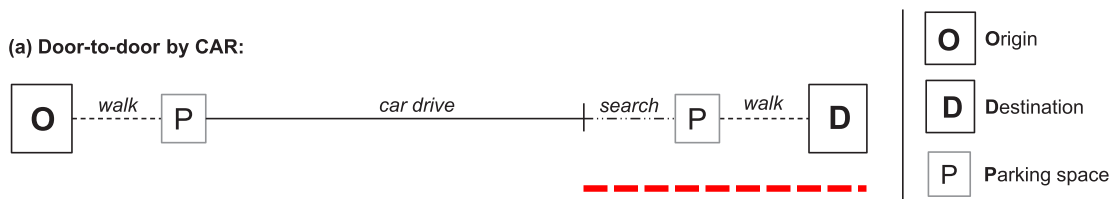
\includegraphics[width=\textwidth]{images/door2door.png}
    \caption[Door-to-door approach]{The entire travel chain of a private car using the door-to-door approach. The red dashed line represents the parking process segment of the travel chain. Figure adapted from Salonen and Toivonen (\citeyear{Salonen2013}).}%
    \label{fig:door-to-door}%
\end{figure}

%\newpage
%\subsection{Parking time estimations}
%\justify
Häyrynen \& Kalenoja's Tampere (\cite{Kalenoja2003})
\item Broad estimations used in Helsinki Travel Time Matrix: item 0.42 min searching for parking, 2 min and 2.5 min walking in TTM18 (\cite{Tenkanen2020})
Donald Shoup's parking time study (\cite{Shoup2006})

%The Helsinki Capital Region faces increasing pressure to manage its traffic because (\textcolor{red}{LÄHDE}). --Semi huono teksti, kokeile vaikka:
To aid Helsinki Capital Region in search for more reality-based parking policy and land use planning, this study produces parking duration data at the granularity of postal code areas.

\newpage
\subsection{Research in parcipatory GIS and map surveys}
\justify
%PPGIS bibliography and map survey considerations
Comparing conventional and PPGIS approaches in measuring equality of access to urban aquatic environments (\cite{Laatikainen2015})
Do suburban residents prefer the fastest or low-carbon travel modes? Combining public participation GIS and multimodal travel time analysis for daily mobility research (\cite{Salonen2014}).